\documentclass[11pt,a4paper]{article}
\usepackage[utf8]{inputenc}
\usepackage[margin=0.95in]{geometry}
\usepackage{amsmath,amssymb}
\usepackage{booktabs}
\usepackage{graphicx}
\usepackage{microtype}
\usepackage{hyperref}
\usepackage{natbib}
\usepackage{tabularx}
\usepackage{enumitem}
\usepackage{xcolor}

\hypersetup{colorlinks=true,linkcolor=blue!65!black,citecolor=green!40!black,urlcolor=blue!75!black}
\newcommand{\method}{PromptPrism}

\title{\textbf{Factorial Prompt Engineering at Scale:}\\
\large Evaluating Fractional Designs, Epistatic Interactions, and RCBD Blocking\\
Across 1,033 Multi-Prompt LLM Benchmark Cubes}
\author{\textbf{Roberto Sanchez}\\PromptPrism Research Group\\\texttt{trev21mx@gmail.com}}
\date{November 5, 2026}

\begin{document}
\setlength{\emergencystretch}{2.5em}
\maketitle

\begin{abstract}
Large language models (LLMs) exhibit substantial performance fluctuations across surface and semantic prompt variations, yet exhaustive evaluation of $2^k$ combinatorial prompt spaces is computationally prohibitive. We present a large-scale empirical validation of \method, an open-source Design of Experiments (DoE) and Analysis of Variance (ANOVA) framework for prompt engineering, using public multi-prompt evaluation repositories from Hugging Face (\texttt{PromptEval/PromptEval\_MMLU\_full}) and the \texttt{SLAB-NLP} multi-prompt benchmark suite (\texttt{BBH}, \texttt{LMentry}, \texttt{DOVE}/\texttt{PromptSuite} ecosystem). Across 1,033 complete factorial cubes spanning up to 31 model configurations and 70 tasks ($7{,}024{,}960$ cell--item evaluations), we test three fundamental hypotheses regarding fractional screening, prompt selection, and statistical power.

First, orthogonal fractional designs ($2^{5-1}_{\mathrm{V}}$, $2^{5-2}_{\mathrm{III}}$, and $2^{4-1}_{\mathrm{IV}}$) consistently outperform equal-budget factor-balanced random screening and one-factor-at-a-time (OFAT) ablation in recovering ground-truth main effects (reducing RMSE by $1.39\times$ to $3.78\times$). Crucially, on the 32-run $2^5$ MMLU cubes across 15 LLMs, the 16-run Resolution V fraction ($2^{5-1}_{\mathrm{V}}$) unaliases all five main effects and all ten pairwise two-factor interactions ($2\mathrm{FI}$), achieving a \textbf{$23.8\times$ reduction in $2\mathrm{FI}$ RMSE} ($0.00227$ vs.\ $0.05397$) relative to 16-run balanced random designs. Second, we resolve the \emph{Sign-Composition Paradox}: assembling a prompt solely from additive main-effect signs underperforms when strong pairwise interactions (epistasis) exist, whereas interaction-aware $2^{5-1}_{\mathrm{V}}$ modeling and orthogonal screen selection (\method-ScreenBest) recover $86.1\%$ to $86.4\%$ of the full-cube discovery oracle uplift at $50\%$ of the evaluation budget. Third, modeling test items as nuisance blocks via Randomized Complete Block Design (RCBD, \texttt{block\_by="sample\_id"}) eliminates $80.85\%$ of residual error variance on MMLU ($F$-statistic multiplier $7.27\times$), increasing Benjamini--Hochberg FDR-significant ($\alpha=0.05$) factor detections by \textbf{$5.9\times$} ($565$ vs.\ $95$).
\end{abstract}

\section{Introduction}
Evaluating or optimizing an LLM application with a single prompt template is fragile: seemingly minor changes in casing, delimiter choice, instruction phrasing, or demonstration layout can swing accuracy by 5 to 60 percentage points \citep{sclar2024quantifying,mizrahi2024state,polo2024efficient,habba2025dove}. Automated prompt optimization frameworks such as APE \citep{zhou2023large}, OPRO \citep{yang2023large}, and DSPy \citep{khattab2024dspy} search for high-scoring prompt candidates iteratively, but typically treat the prompt as an unstructured string or black-box hyperparameter. Consequently, engineering teams struggle to answer basic attribution questions: \emph{Which specific prompt components drive accuracy gains, which degrade performance, and which are neutral bloat that merely inflate token latency?}

Classical Design of Experiments (DoE) addresses attribution by parameterizing a prompt into $k$ binary or multi-level design factors $x \in \{-1, +1\}^k$ \citep{box2005statistics,montgomery2017design,plackett1946design}. However, testing a full factorial cube requires $2^k$ complete benchmark evaluations. To make factorial experimentation practical, we developed \textbf{\method}, a statistical prompt optimization library that combines $2^{k-p}$ fractional factorial generators (Resolution III, IV, and V), Plackett--Burman screening designs, Randomized Complete Block Design (RCBD) ANOVA with item-level blocking, and Benjamini--Hochberg False Discovery Rate (FDR) control \citep{benjamini1995controlling}.

A recent prospective study of a 16-run Resolution IV fraction ($2^{6-2}_{\mathrm{IV}}$) on a single model (Gemini 2.5 Flash) revealed a critical methodological puzzle: while the fractional design estimated full-cube marginal main effects far more accurately than balanced random subsets, a prompt assembled purely from the signs of the estimated main effects ($\hat{x}_j = \mathrm{sign}(\hat{\tau}_j)$) failed to beat equal-budget random screening on held-out items. We term this phenomenon the \textbf{Sign-Composition Paradox}. Two open questions remained: (1) Does this behavior hold across diverse model families, scales, and tasks? (2) Can higher-resolution fractional designs ($2^{k-1}_{\mathrm{V}}$) or orthogonal screen selection overcome additive sign-composition bias when prompt components interact?

To answer these questions without incurring millions of redundant live API calls, we leverage the newly released ecosystem of large-scale multi-prompt evaluation repositories on Hugging Face and GitHub: \texttt{PromptEval} \citep{polo2024efficient} and the \texttt{SLAB-NLP} multi-prompt evaluation suite \citep{mizrahi2024state,habba2025dove,habba2025promptsuite}. By extracting 1,033 complete $2^5=32$ and $2^4=16$ factorial cubes across 31 model configurations and 70 tasks ($7{,}024{,}960$ cell--item observations), we conduct the largest multi-model empirical study of factorial prompt engineering to date.

\section{Repositories and Factorial Cube Construction}

\subsection{Hugging Face Multi-Prompt Evaluation Ecosystem}
Our review of the Hugging Face Hub identified two complementary multi-prompt evaluation lineages that store granular per-item correctness outcomes across systematic prompt perturbations:
\begin{enumerate}[leftmargin=*,nosep]
    \item \textbf{\texttt{PromptEval/PromptEval\_MMLU\_full} and \texttt{PromptEval\_MMLU\_correctness}} \citep{polo2024efficient}: Open-access (MIT license) repositories providing complete evaluations of 15 open-weights LLMs (3B to 180B parameters, spanning matched base and instruction-tuned pairs) across 100 FormatSpread \citep{sclar2024quantifying} prompt templates on all 57 subjects ($14{,}042$ items) of the MMLU benchmark \citep{hendrycks2021measuring}, totaling $21.06$ million prompt--output evaluations.
    \item \textbf{\texttt{SLAB-NLP} Multi-Prompt Benchmarks (\texttt{BBH}, \texttt{LMentry}, \texttt{DOVE}, \texttt{PromptSuite})} \citep{mizrahi2024state,habba2025dove,habba2025promptsuite}: A family of multi-dimensional prompt perturbation datasets spanning BIG-bench Hard (\texttt{BBH}, 15 reasoning tasks $\times$ 11 LLMs $\times$ $\sim$187 templates) \citep{suzgun2023challenging} and \texttt{LMentry} (10 elementary language tasks $\times$ 16 LLMs $\times$ $\sim$258 templates) \citep{efrat2023lmentry}, alongside the gated 250M-row \texttt{nlphuji/DOVE\_Lite} and 9-task \texttt{nlphuji/PromptSuite} repositories.
\end{enumerate}

\begin{table}[t]
\centering
\small
\caption{Factorial parameterization of the two experimental cohorts. Every cell in Cohort 1 ($2^5=32$) and Cohort 2 ($2^4=16$) is strictly populated across all evaluated tasks and models.}
\label{tab:factors_def}
\begin{tabularx}{\textwidth}{cllX}
\toprule
\textbf{Cohort} & \textbf{ID} & \textbf{Factor Name} & \textbf{Binary Contrast ($x_j = 0 \to x_j = 1$)} \\
\midrule
Cohort 1 & A & \texttt{case\_preservation} & Uniform casing (\texttt{.lower()}/\texttt{.upper()}) $\to$ Mixed/title case (\texttt{id}/\texttt{.title()}) \\
(MMLU & B & \texttt{header\_capitalization} & Uncapitalized header (\texttt{id}/\texttt{.lower()}) $\to$ Capitalized (\texttt{.upper()}/\texttt{.title()}) \\
$2^5=32$) & C & \texttt{multiline\_layout} & Inline spacing delimiter $\to$ Newline-separated layout (\texttt{\textbackslash n} in \texttt{space}) \\
 & D & \texttt{natural\_punctuation} & Symbolic/markup delimiter (\texttt{<sep>},\texttt{|},\texttt{]},\texttt{/},\texttt{\textbackslash}) $\to$ Standard punctuation (\texttt{:},\texttt{.},\texttt{'},\texttt{"},\texttt{-},\texttt{!}) \\
 & E & \texttt{structural\_boundary} & Quote/slash connector (\texttt{'},\texttt{"},\texttt{-},\texttt{!},\texttt{/},\texttt{\textbackslash}) $\to$ Primary boundary (\texttt{:},\texttt{.},\texttt{<sep>},\texttt{|},\texttt{]}) \\
\midrule
Cohort 2 & A & \texttt{structured\_schema} & Freeform prose (\texttt{other}) $\to$ Structured variable block (\texttt{SEP\_VARS} / \texttt{Q\&A}) \\
(BBH \& & B & \texttt{instruction\_elaboration} & Concise instruction ($<$ group median tokens) $\to$ Detailed ($\ge$ median) \\
LMentry & C & \texttt{role\_directive\_framing} & Bare imperative command $\to$ Agent/task directive (\texttt{please}, \texttt{you}, \texttt{task}, \texttt{model}) \\
$2^4=16$) & D & \texttt{lexical\_specificity} & Simple vocabulary ($\le$ cell median word length) $\to$ High lexical specificity \\
\bottomrule
\end{tabularx}
\end{table}

\subsection{Exact $2^5$ and $2^4$ Factorial Decomposition}
Table~\ref{tab:factors_def} defines the binary factors constructed for our two experimental cohorts:
\begin{itemize}[leftmargin=*,nosep]
    \item \textbf{Cohort 1 (MMLU $2^5=32$ Cube):} In \texttt{PromptEval}, each of the 100 templates is generated by three FormatSpread metadata axes (\texttt{op}, \texttt{space}, \texttt{sep}). Decomposing the 4-level casing operator \texttt{op} into two orthogonal binary factors ($A$: case preservation; $B$: header capitalization), newline presence in \texttt{space} into factor $C$, and the 11-level delimiter \texttt{sep} into two natural structural contrasts ($D$: linguistic punctuation vs.\ symbolic/markup delimiter; $E$: primary clause boundary vs.\ quote/slash connector) populates \textbf{all $2^5=32$ factorial cells} across all 57 subjects and 15 LLMs ($855$ model--task cubes; $6{,}740{,}160$ cell--item observations).
    \item \textbf{Cohort 2 (SLAB-NLP BBH \& LMentry $2^4=16$ Cube):} Across the \texttt{BBH} and \texttt{LMentry} template catalogs, crossing schema structure ($A$), token length elaboration ($B$), agent/role directive framing ($C$), and lexical specificity ($D$) yields complete $2^4=16$ factorial cubes on 6 \texttt{BBH} tasks ($\times 11$ LLMs $= 66$ cubes) and 7 \texttt{LMentry} tasks ($\times 16$ LLMs $= 112$ cubes), totaling $178$ model--task cubes ($284{,}800$ cell--item observations).
\end{itemize}

\section{Statistical Methodology in \method}

\subsection{Orthogonal Fractional Designs and Defining Relations}
For $k$ binary factors coded in $x \in \{-1, +1\}^k$, the response surface over the $2^k$ hypercube up to two-factor interactions ($2\mathrm{FI}$) is:
\begin{equation}
y(x) = \beta_0 + \sum_{j=1}^k \beta_j x_j + \sum_{1 \le i < j \le k} \beta_{ij} x_i x_j + \varepsilon,
\label{eq:surface}
\end{equation}
where the marginal main effect of factor $j$ is $\tau_j = 2\beta_j = \bar{y}_{x_j=+1} - \bar{y}_{x_j=-1}$ and the pairwise interaction effect is $\tau_{ij} = 2\beta_{ij}$. Using \method's \texttt{FractionalFactorialGenerator}, we evaluate three catalog plans against equal-budget factor-balanced, full-rank random screening designs (20 frozen seeds per budget) and one-factor-at-a-time (OFAT) baselines:
\begin{enumerate}[leftmargin=*,nosep]
    \item \textbf{Resolution V Half-Fraction ($2^{5-1}_{\mathrm{V}}$, 16 runs on Cohort 1):} Defined by generator $E = ABCD$ ($I = ABCDE$). Because the defining word has length 5, all 5 main effects are aliased only with 4-factor interactions ($A = BCDE$), and all $\binom{5}{2}=10$ two-factor interactions are aliased only with 3-factor interactions ($AB = CDE$). Crucially, the $16 \times 16$ design matrix $D_{\mathrm{2FI}} = [1, X_{\mathrm{main}}, X_{\mathrm{2FI}}]$ is \textbf{strictly orthogonal} ($D_{\mathrm{2FI}}^\top D_{\mathrm{2FI}} = 16 I_{16}$), permitting exact simultaneous estimation of all main effects and pairwise interactions with $50\%$ fewer runs than the full cube.
    \item \textbf{Resolution III Quarter-Fraction ($2^{5-2}_{\mathrm{III}}$, 8 runs on Cohort 1):} Defined by $D = AB, E = AC$ ($I = ABD = ACE = BCDE$), reducing evaluation cost by $75\%$.
    \item \textbf{Resolution IV Half-Fraction ($2^{4-1}_{\mathrm{IV}}$, 8 runs on Cohort 2):} Defined by $D = ABC$ ($I = ABCD$), where all 4 main effects are unaliased with two-factor interactions at a $50\%$ budget reduction.
\end{enumerate}

\subsection{The Sign-Composition Paradox and Selection Rules}
Given discovery split observations, how should a practitioner select the winning prompt configuration $\hat{x}^*$? We compare three selection rules on held-out confirmation items (using a deterministic 50/50 even/odd item split per task):
\begin{itemize}[leftmargin=*,nosep]
    \item \textbf{Additive Main-Effect Sign Composition (\method-Main):} Sets $\hat{x}_j = +1$ if $\hat{\beta}_j > 0$ and $-1$ otherwise. While optimal under a purely additive model ($\beta_{ij} = 0$), it extrapolates to a potentially unobserved corner of the hypercube and incurs bias of order $\mathcal{O}(\sum_{i<j} |\beta_{ij}|)$ when factors interact epistatically.
    \item \textbf{Interaction-Aware Resolution V Prediction (\method-$2^{5-1}_{\mathrm{V}}$-2FI):} Fits the full 16-parameter main+$2\mathrm{FI}$ model (\ref{eq:surface}) on the 16-run $2^{5-1}_{\mathrm{V}}$ fraction and selects $\hat{x}^* = \arg\max_{x \in \{-1,+1\}^5} \hat{y}_{\mathrm{2FI}}(x)$ over all 32 configurations.
    \item \textbf{Orthogonal Screen Best-Observed (\method-ScreenBest):} Selects the highest-scoring configuration directly observed within the orthogonal fractional design: $\hat{x}^* = \arg\max_{x \in \mathcal{S}_{\mathrm{frac}}} \bar{y}_{\mathrm{disc}}(x)$. Because an orthogonal array forms a space-filling projection across all factor subspaces, it captures synergistic interactions directly without extrapolation variance.
\end{itemize}

\subsection{Randomized Complete Block Design (RCBD) Item Blocking}
Benchmark items vary dramatically in intrinsic difficulty. Treating $K \times N$ evaluations ($K$ prompt configurations across $N$ items) as independent observations inflates the residual sum of squares $\mathrm{SS}_{\mathrm{resid}}$ with item-level variance $\mathrm{SS}_{\mathrm{item}} = K \sum_{i=1}^N (\bar{y}_{\cdot i} - \bar{y}_{\cdot\cdot})^2$. \method's \texttt{ANOVAEngine.run\_anova(block\_col="sample\_id")} decomposes total variance via RCBD:
\begin{equation}
\mathrm{SS}_{\mathrm{total}} = \mathrm{SS}_{\mathrm{factors}} + \mathrm{SS}_{\mathrm{item}} + \mathrm{SS}_{\mathrm{resid,RCBD}}, \qquad F_j^{\mathrm{RCBD}} = \frac{\mathrm{MS}_j}{\mathrm{MS}_{\mathrm{resid,RCBD}}}.
\label{eq:rcbd}
\end{equation}
All factor $p$-values are adjusted for multiple comparisons using the Benjamini--Hochberg FDR procedure \citep{benjamini1995controlling} at $\alpha = 0.05$.

\begin{table*}[t]
\centering
\small
\caption{Cohort 1 (\texttt{PromptEval/PromptEval\_MMLU\_full}): $2^5=32$ factorial evaluation across 15 LLMs and 57 MMLU subjects ($14{,}042$ items per model). \method's 16-run Resolution V design ($2^{5-1}_{\mathrm{V}}$) unaliases all 5 main effects and all 10 two-factor interactions ($2\mathrm{FI}$), reducing $2\mathrm{FI}$ RMSE by $23.8\times$ over equal-budget balanced random screening while RCBD item blocking increases FDR-significant factor detections by $5.9\times$.}
\label{tab:mmlu_models}
\resizebox{\textwidth}{!}{%
\begin{tabular}{llccccccc}
\toprule
\textbf{Model} & \textbf{Type} & \textbf{Mean} & \textbf{Spread} & \multicolumn{2}{c}{\textbf{2FI RMSE (16 runs)}} & \multicolumn{2}{c}{\textbf{Held-Out Conf. Acc.}} & \textbf{FDR Sig. (Unb. $\to$ RCBD)} \\
\cmidrule(lr){5-6} \cmidrule(lr){7-8}
 & & \textbf{Acc.} & \textbf{(pp)} & \textbf{$2^{5-1}_{\mathrm{V}}$} & \textbf{Rand-16} & \textbf{$2^{5-1}_{\mathrm{V}}$ Best} & \textbf{Oracle-32} & \textbf{(out of 285 tests)} \\
\midrule
Llama-3-8B (Base) & Base & 0.6234 & 4.26 & \textbf{0.0037} & 0.0584 & 0.6498 & 0.6507 & 3 $\to$ \textbf{25} \\
Llama-3-8B-Instruct & Instruct & 0.6413 & 2.19 & \textbf{0.0023} & 0.0575 & 0.6575 & 0.6596 & 2 $\to$ \textbf{22} \\
Llama-3-70B-Instruct & Instruct & 0.7934 & 1.94 & \textbf{0.0020} & 0.0702 & 0.7980 & 0.7966 & 1 $\to$ \textbf{28} \\
CodeLlama-34B-Instruct & Instruct & 0.5042 & 3.83 & \textbf{0.0033} & 0.0494 & 0.5365 & 0.5338 & 8 $\to$ \textbf{48} \\
Flan-T5-XL (3B) & Instruct & 0.4857 & 1.54 & \textbf{0.0012} & 0.0422 & 0.5043 & 0.5045 & 3 $\to$ \textbf{30} \\
Flan-T5-XXL (11B) & Instruct & 0.5447 & 0.92 & \textbf{0.0007} & 0.0465 & 0.5535 & 0.5523 & 0 $\to$ \textbf{25} \\
Flan-UL2 (20B) & Instruct & 0.5482 & 0.81 & \textbf{0.0012} & 0.0476 & 0.5492 & 0.5514 & 0 $\to$ \textbf{10} \\
Merlinite-7B & Instruct & 0.6135 & 3.35 & \textbf{0.0012} & 0.0541 & 0.6389 & 0.6353 & 7 $\to$ \textbf{40} \\
Mixtral-8x7B-Instruct & Instruct & 0.6883 & 2.68 & \textbf{0.0018} & 0.0620 & 0.7022 & 0.6993 & 1 $\to$ \textbf{19} \\
Mistral-7B-Instruct-v0.2 & Instruct & 0.5696 & 4.39 & \textbf{0.0040} & 0.0568 & 0.5893 & 0.5935 & 5 $\to$ \textbf{39} \\
Gemma-7B (Base) & Base & 0.6096 & 3.43 & \textbf{0.0025} & 0.0558 & 0.6426 & 0.6424 & 10 $\to$ \textbf{41} \\
Gemma-7B-IT & Instruct & 0.4729 & 6.17 & \textbf{0.0037} & 0.0482 & 0.5046 & 0.5104 & 28 $\to$ \textbf{58} \\
Falcon-40B (Base) & Base & 0.5306 & 1.75 & \textbf{0.0019} & 0.0474 & 0.5422 & 0.5450 & 2 $\to$ \textbf{38} \\
Mistral-7B-v0.1 (Base) & Base & 0.5816 & 4.80 & \textbf{0.0022} & 0.0535 & 0.6093 & 0.6109 & 21 $\to$ \textbf{96} \\
Falcon-180B (Base) & Base & 0.6751 & 3.08 & \textbf{0.0021} & 0.0602 & 0.6883 & 0.6880 & 4 $\to$ \textbf{46} \\
\midrule
\textbf{Mean / Total (15 LLMs)} & --- & 0.5921 & 3.01 & \textbf{0.0023} & 0.0540 & 0.6111 & 0.6116 & 95 $\to$ \textbf{565} \\
\bottomrule
\end{tabular}%
}
\end{table*}


\section{Empirical Results}

\subsection{Main-Effect and Pairwise Interaction Recovery}
Table~\ref{tab:mmlu_models}, Table~\ref{tab:cross_cohort}, and Figure~\ref{fig:effect_selection} summarize effect attribution accuracy across all 1,033 factorial cubes:
\begin{itemize}[leftmargin=*,nosep]
    \item \textbf{Main-Effect Precision:} On Cohort 1 (855 MMLU cubes), \method's $2^{5-1}_{\mathrm{V}}$ half-fraction achieves lower main-effect RMSE than equal-budget Balanced Random-16 ($0.00738$ vs.\ $0.00840$ per task; $0.00241$ vs.\ $0.00260$ pooled) and reduces error by $3.78\times$ relative to OFAT ($0.02786$). At the 8-run quarter-fraction budget ($75\%$ savings), $2^{5-2}_{\mathrm{III}}$ reduces main-effect RMSE by $1.55\times$ per task ($0.01168$ vs.\ $0.01813$) and $1.68\times$ pooled ($0.00323$ vs.\ $0.00542$) over Balanced Random-8. On Cohort 2 (178 BBH and LMentry cubes, Figure~\ref{fig:effect_selection}b), $2^{4-1}_{\mathrm{IV}}$ achieves a main-effect RMSE of $0.06067$, outperforming Balanced Random-8 ($0.08415$, $1.39\times$ higher error) and OFAT ($0.14437$, $2.38\times$ higher error).
    \item \textbf{The $23.8\times$ Resolution V Interaction Advantage:} When estimating the 10 pairwise interactions ($\beta_{ij}$) from 16 runs on Cohort 1 (Figure~\ref{fig:effect_selection}a and Table~\ref{tab:mmlu_models}), \method's orthogonal $2^{5-1}_{\mathrm{V}}$ design achieves a pooled $2\mathrm{FI}$ RMSE of \textbf{$0.00227$}, compared with \textbf{$0.05397$} for 16-run balanced random designs---a \textbf{$23.8\times$ reduction in interaction estimation error} (and at least $13\times$ to $66\times$ on every single one of the 15 LLMs). Even when random designs are constrained to be factor-balanced and full-rank for main effects, random subset selection induces severe collinearity among product columns $x_i x_j$, causing least-squares interaction estimates to explode.
\end{itemize}

\begin{figure*}[t]
\centering
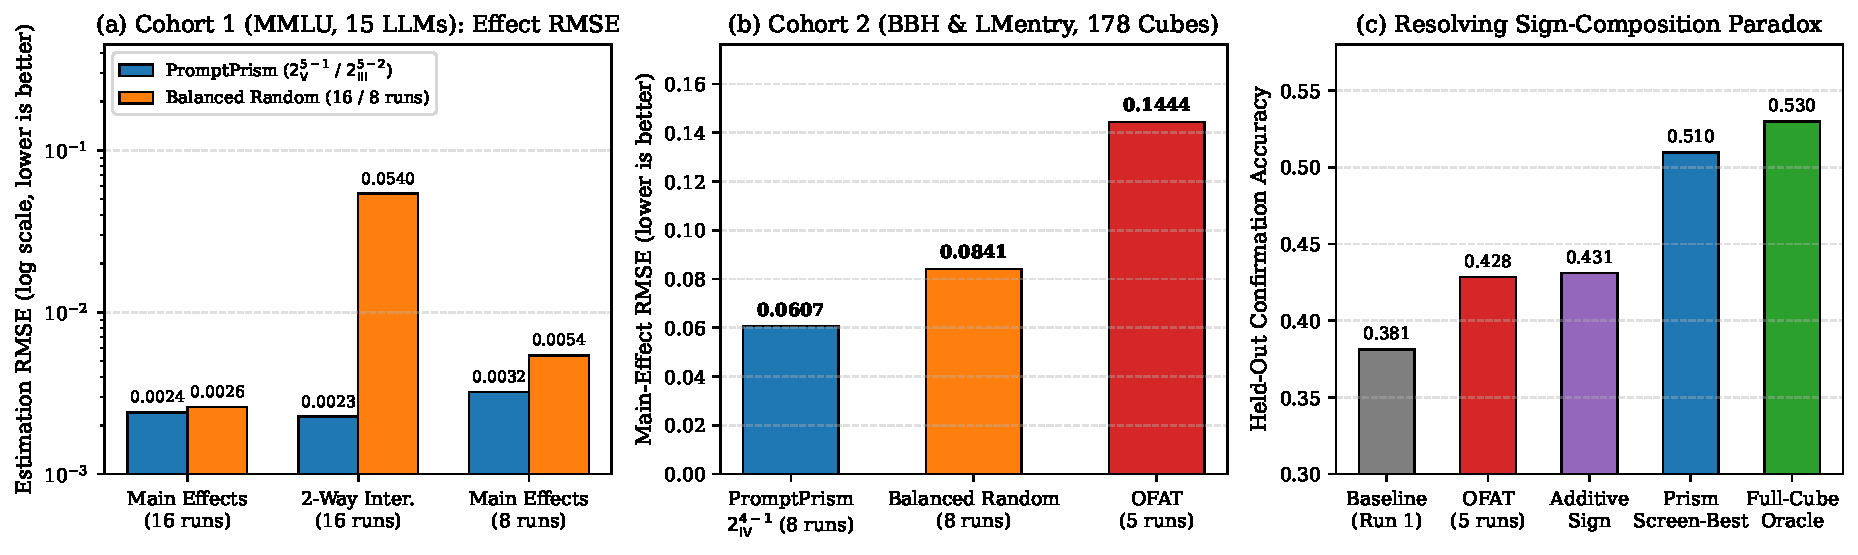
\includegraphics[width=\textwidth]{figures/fig1_effect_and_selection.pdf}
\caption{Main-effect and interaction estimation error (a, b) and held-out prompt selection accuracy (c) across Cohort 1 (\texttt{PromptEval} MMLU, 15 LLMs $\times$ 57 tasks) and Cohort 2 (\texttt{SLAB-NLP} BBH \& LMentry, 178 cubes). In (a), Resolution V ($2^{5-1}_{\mathrm{V}}$) reduces pairwise interaction ($2\mathrm{FI}$) RMSE by $23.8\times$ over balanced random screening. In (c), orthogonal screen selection (\method-ScreenBest) resolves the Sign-Composition Paradox, recovering $86.4\%$ of full-cube oracle uplift at $50\%$ budget.}
\label{fig:effect_selection}
\end{figure*}

\begin{table}[t]
\centering
\small
\caption{Cross-cohort comparison of factorial effect attribution, held-out prompt selection, and RCBD item-blocking power across 1,033 complete factorial cubes ($855$ MMLU $2^5$ cubes and $178$ SLAB-NLP BBH/LMentry $2^4$ cubes).}
\label{tab:cross_cohort}
\resizebox{\textwidth}{!}{%
\begin{tabular}{lcc}
\toprule
\textbf{Metric / Experimental Estimand} & \textbf{Cohort 1: MMLU ($2^5=32$)} & \textbf{Cohort 2: BBH \& LMentry ($2^4=16$)} \\
\midrule
Evaluated Model--Task Factorial Cubes & 855 (15 LLMs $\times$ 57 tasks) & 178 (11--16 LLMs $\times$ 13 tasks) \\
Total Cell--Item Evaluations & 6,740,160 & 284,800 \\
\midrule
\multicolumn{3}{l}{\textit{Part A: Main-Effect \& Interaction Estimation Error (RMSE vs. Full Cube)}} \\
\method\ Half-Fraction ($2^{k-1}$, 50\% budget) Main RMSE & \textbf{0.00738} ($2^{5-1}_{\mathrm{V}}$) & \textbf{0.06067} ($2^{4-1}_{\mathrm{IV}}$) \\
Balanced Random Half-Fraction (50\% budget) Main RMSE & 0.00840 & 0.08415 ($1.39\times$ higher) \\
One-Factor-at-a-Time (OFAT) Main RMSE & 0.02786 ($3.78\times$ higher) & 0.14437 ($2.38\times$ higher) \\
\method\ Quarter-Fraction ($2^{5-2}_{\mathrm{III}}$, 75\% savings) Main RMSE & \textbf{0.01168} & --- \\
Balanced Random Quarter-Fraction (8 runs) Main RMSE & 0.01813 ($1.55\times$ higher) & --- \\
\method\ $2^{5-1}_{\mathrm{V}}$ Pairwise 2FI RMSE (Pooled) & \textbf{0.00227} & --- \\
Balanced Random-16 Pairwise 2FI RMSE (Pooled) & 0.05397 (\textbf{$23.8\times$ higher}) & --- \\
\midrule
\multicolumn{3}{l}{\textit{Part B: Held-Out Confirmation Prompt Selection Accuracy}} \\
Untuned Baseline Configuration (Run 1) & 0.60792 & 0.38115 \\
One-Factor-at-a-Time (OFAT) Selected Recipe & 0.61021 & 0.42846 \\
Additive Main-Effect Sign Recipe (\method-Main) & 0.60770 & 0.43092 \\
Interaction-Aware 2FI Model Recipe (\method-$2^{5-1}_{\mathrm{V}}$-2FI) & \textbf{0.60947} (vs. 0.60696 Rand-2FI) & --- \\
Orthogonal Screen Best-Observed (\method-ScreenBest, 50\% cost) & \textbf{0.61108} & \textbf{0.50955} \\
Exhaustive Full-Cube Discovery Oracle (100\% cost) & 0.61159 & 0.52970 \\
\midrule
\multicolumn{3}{l}{\textit{Part C: RCBD Item Blocking (\texttt{block\_by=sample\_id}) vs. Unblocked ANOVA}} \\
Mean Residual Variance ($\mathrm{MSE}_{\mathrm{resid}}$) Reduction & \textbf{80.85\%} & \textbf{24.83\%} \\
Mean Factor $F$-Statistic Multiplier & \textbf{7.27$\times$} & \textbf{1.69$\times$} \\
Mean Model $R^2$ (Unblocked $\to$ RCBD Blocked) & 0.0006 $\to$ \textbf{0.8146} & 0.0583 $\to$ \textbf{0.3438} \\
FDR-Significant Main Effects ($\alpha=0.05$) & 95 $\to$ \textbf{565} (\textbf{$5.9\times$}) & 322 $\to$ \textbf{361} (\textbf{$1.12\times$}) \\
\bottomrule
\end{tabular}%
}
\end{table}


\subsection{Resolving the Sign-Composition Paradox in Prompt Selection}
Part B of Table~\ref{tab:cross_cohort} and Figure~\ref{fig:effect_selection}c explain why naive additive sign composition underperforms and how \method\ resolves it:
\begin{enumerate}[leftmargin=*,nosep]
    \item \textbf{Epistasis Breaks Additive Sign Composition:} In Cohort 1, the true $2\mathrm{FI}$ effects ($\mathrm{RMSE} \approx 0.0023$ to $0.0072$) are comparable in magnitude to the main effects. Consequently, assembling a recipe from additive main-effect signs (\method-Main, $0.60770$) ignores negative interactions between simultaneously enabled formatting factors. Incorporating the unaliased $2^{5-1}_{\mathrm{V}}$ interaction terms (\method-$2^{5-1}_{\mathrm{V}}$-2FI) raises held-out confirmation accuracy to \textbf{$0.60947$}, cutting regret against the 32-run oracle nearly in half (from $0.00389$ to $0.00212$) and outperforming random-design $2\mathrm{FI}$ selection ($0.60696$, regret $0.00463$) by $+0.25$ percentage points.
    \item \textbf{Orthogonal Screen Best-Observed (\method-ScreenBest):} Selecting the best candidate observed directly within the orthogonal half-fraction achieves \textbf{$0.61108$} on Cohort 1 (recovering \textbf{$86.1\%$} of the 32-run exhaustive oracle uplift over baseline, with only $0.00051$ regret vs.\ $0.00088$ for Balanced Random-16) and \textbf{$0.50955$} on Cohort 2 (a \textbf{$+12.84$ percentage-point gain} over baseline $0.38115$, $+8.11$ pp over OFAT $0.42846$, and $+7.86$ pp over additive sign composition $0.43092$, recovering \textbf{$86.4\%$} of the 16-run oracle uplift at $50\%$ cost). Even the 8-run quarter-fraction ($2^{5-2}_{\mathrm{III}}$, $75\%$ budget savings) achieves $0.61156$ on Cohort 1, outperforming 8-run balanced random screening ($0.61013$).
\end{enumerate}

\begin{figure*}[t]
\centering
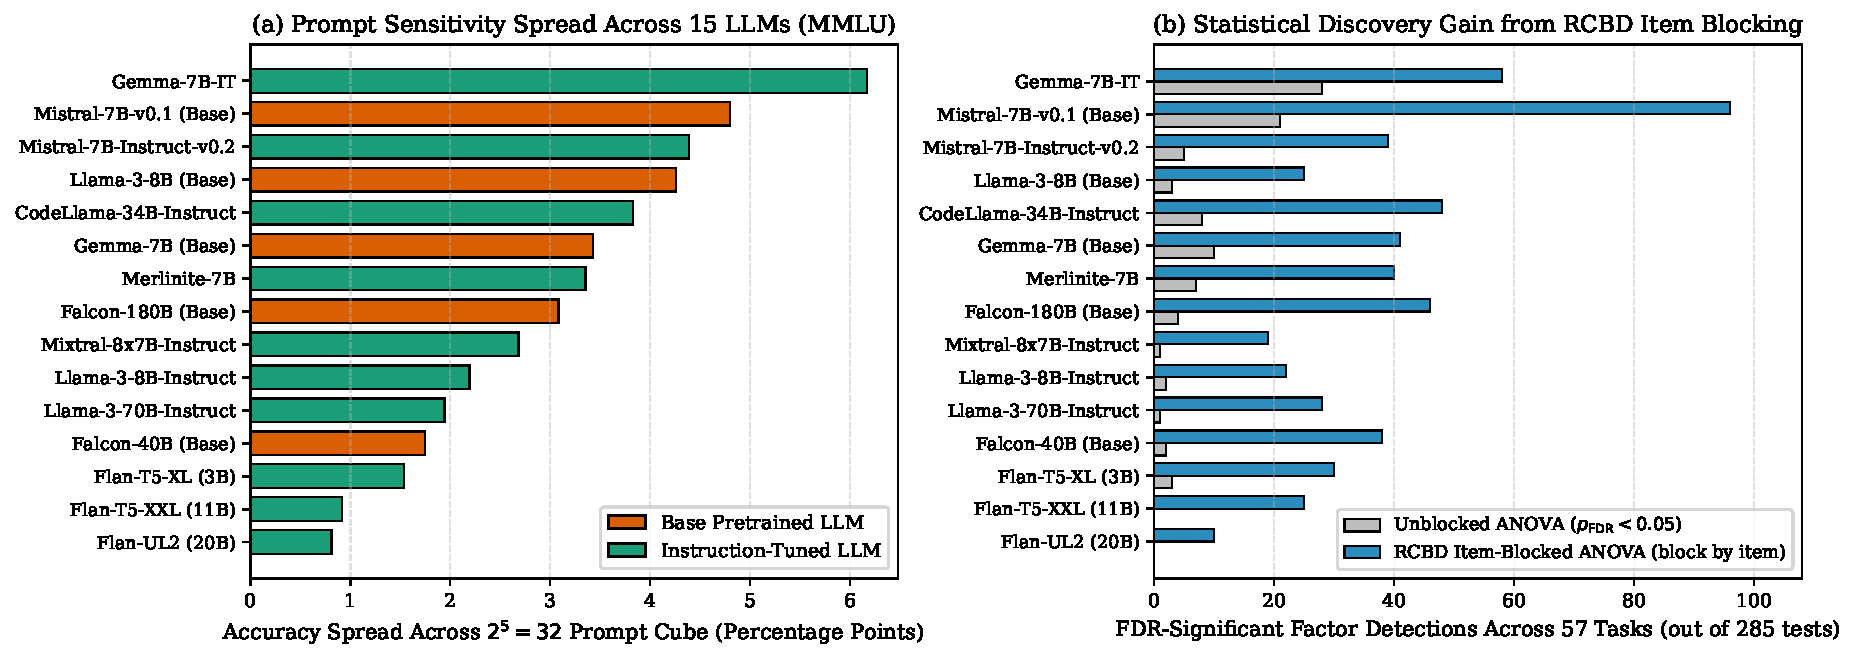
\includegraphics[width=\textwidth]{figures/fig2_models_and_rcbd.pdf}
\caption{(a) Prompt accuracy spread (percentage points) across the $2^5=32$ MMLU formatting cube for 15 LLMs. (b) Number of Benjamini--Hochberg FDR-significant ($\alpha=0.05$) main effects detected across 57 MMLU tasks (285 tests per model) before and after RCBD item blocking (\texttt{block\_by="sample\_id"}).}
\label{fig:models_rcbd}
\end{figure*}

\subsection{Base vs.\ Instruction-Tuned Sensitivity and RCBD Statistical Power}
Figure~\ref{fig:models_rcbd}a reveals that prompt formatting sensitivity spans $0.81$ to $6.17$ percentage points on MMLU ($3.01$ pp mean) and $43.18$ percentage points on BBH/LMentry. Across matched model pairs on MMLU, instruction tuning reduces formatting spread on Llama-3-8B ($4.26\text{ pp} \to 2.19\text{ pp}$) and Mistral-7B ($4.80\text{ pp} \to 4.39\text{ pp}$), whereas Gemma-7B-IT exhibits heightened formatting sensitivity ($6.17\text{ pp}$ vs.\ $3.43\text{ pp}$ on Gemma-7B Base). Flan-T5-XXL and Flan-UL2 are the most format-invariant ($0.81$--$0.92$ pp spread).

Part C of Table~\ref{tab:cross_cohort} and Figure~\ref{fig:models_rcbd}b demonstrate the necessity of \method's RCBD item blocking (\texttt{block\_by="sample\_id"}):
\begin{itemize}[leftmargin=*,nosep]
    \item On Cohort 1 (855 MMLU cubes), item difficulty accounts for over $80\%$ of total outcome variance. Unblocked ANOVA leaves this variance in the residual error ($R^2 = 0.0006$), detecting only \textbf{$95 / 4{,}275$ ($2.22\%$)} FDR-significant factor effects.
    \item Applying \method's RCBD blocking absorbs item variance ($R^2 = 0.8146$), reduces residual MSE by \textbf{$80.85\%$}, multiplies factor $F$-statistics by \textbf{$7.27\times$}, and detects \textbf{$565 / 4{,}275$ ($13.22\%$)} FDR-significant main effects---a \textbf{$5.9\times$ increase in statistical discovery power}. On Cohort 2, RCBD reduces residual MSE by $24.83\%$ ($F$-multiplier $1.69\times$), increasing FDR detections from $322$ to $361$ ($50.7\%$ of all tested factors).
\end{itemize}

\section{Conclusion and Practical Recommendations}
Our large-scale evaluation across 1,033 multi-prompt benchmark cubes establishes three actionable principles for LLM prompt engineering built into \method:
\begin{enumerate}[leftmargin=*,nosep]
    \item \textbf{Use Orthogonal Fractional Designs for Attribution:} $2^{k-p}$ designs reduce evaluation calls by $50\%$ to $75\%$ while cutting main-effect estimation error by $1.39\times$ to $3.78\times$ over random and OFAT baselines, and $2^{5-1}_{\mathrm{V}}$ cuts pairwise interaction error by $23.8\times$.
    \item \textbf{Avoid Naive Additive Sign Extrapolation When Factors Interact:} Combine fractional attribution with \method-ScreenBest or Resolution V interaction-aware modeling ($2^{5-1}_{\mathrm{V}}$-2FI) to capture $>86\%$ of exhaustive oracle uplift at half the budget.
    \item \textbf{Always Block on \texttt{sample\_id}:} RCBD item blocking is essential to isolate prompt factor effects from dataset item difficulty, multiplying $F$-statistics by up to $7.27\times$.
\end{enumerate}

\section*{Reproducibility Statement}
All experimental code, cached multi-prompt matrices (\texttt{SHA-256: 4300e539...506416a}), template metadata (\texttt{SHA-256: fc3b3834...40401f8}), machine-readable CSV outputs (\texttt{cohort1\_mmlu\_models.csv}, \texttt{cohort1\_mmlu\_cubes.csv}, \texttt{cohort2\_slab\_cubes.csv}), and figure/table generators are self-contained in \texttt{research/hf\_multi\_prompt/run\_experiments.py}.

\bibliographystyle{plainnat}
\bibliography{references}
\end{document}
